\documentclass[a4paper,11pt]{jsarticle}


% 数式
\usepackage{amsmath,amsfonts}
\usepackage{bm}
\usepackage{physics}
% 画像
\usepackage[dvipdfmx]{graphicx}
% ローマ数字
\usepackage{otf}
% 単位
\usepackage{siunitx}
% 表
\usepackage{multirow}
% 化学反応
\usepackage[version=4]{mhchem}
\usepackage{url}

\begin{document}

\title{電子回路論 後半レポート}
\author{05-211525 齋藤駿一}
\date{\today}
\maketitle

本レポートでは,課題1のB,つまり標準ロジックICを用いた8ビット減算回路の回路図の設計に取り組んだ.

\section{半減算器}
ロジックICとして,XOR,インバーター(NOT),ANDの3種類を用いる.

まず,半減算器の回路図は図\ref{fig:HS}のようになる.
以下ではこれをHSブロックとして略記する.

\begin{figure}[htbp]
  \centering
  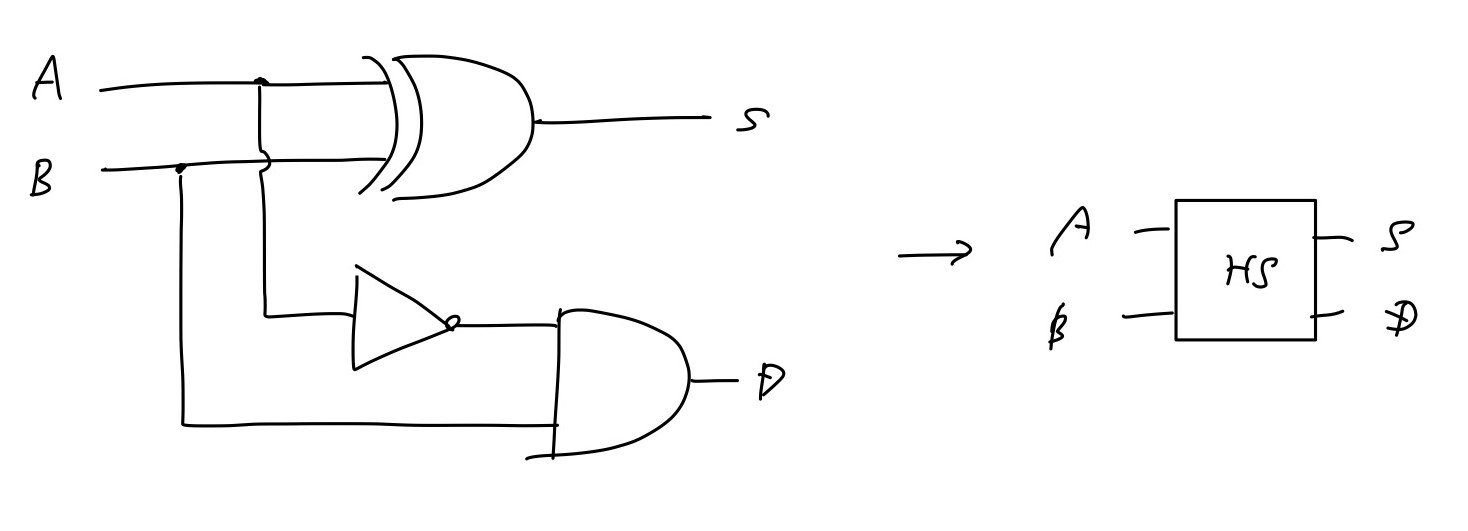
\includegraphics[width=10cm]{HS.jpg}
  \caption{半減算器の回路図.}
  \label{fig:HS}
\end{figure}

半減算器の真理値表は表\ref{tab:HS}のようになる.
\begin{table}[htbp]
  \centering
  \caption{半減算器の真理値表.}
  \label{tab:HS}
  \begin{tabular}{cc|cc}
    \hline
    \multicolumn{2}{c|}{入力} & \multicolumn{2}{c}{出力} \\
    \hline
    A & B & S & D \\
    \hline\hline
    0 & 0 & 0 & 0 \\
    0 & 1 & 1 & 1 \\
    1 & 0 & 1 & 0 \\
    1 & 1 & 0 & 0 \\
    \hline
  \end{tabular}
\end{table}

\section{全減算器}
次に,全減算器の回路図は図\ref{fig:FS}のようになる.
以下ではこれをFSブロックとして略記する.

\begin{figure}[htbp]
  \centering
  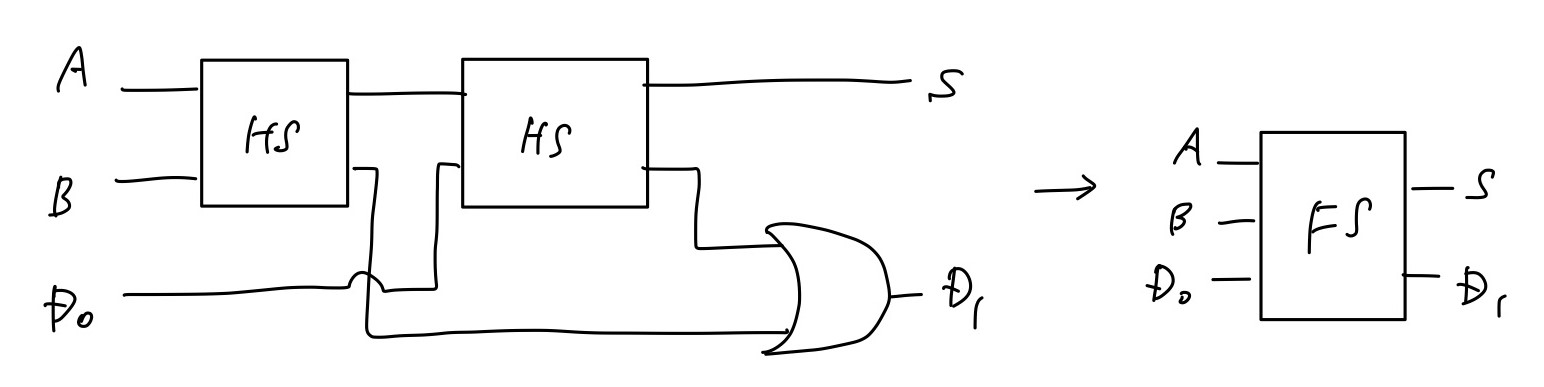
\includegraphics[width=10cm]{FS.jpg}
  \caption{全減算器の回路図.}
  \label{fig:FS}
\end{figure}

全減算器の真理値表は表\ref{tab:FS}のようになる.
\begin{table}[htbp]
  \centering
  \caption{半減算器の真理値表.}
  \label{tab:FS}
  \begin{tabular}{ccc|cc}
    \hline
    \multicolumn{3}{c|}{入力} & \multicolumn{2}{c}{出力} \\
    \hline
    A & B & D0 & S & D1 \\
    \hline\hline
    0 & 0 & 0 & 0 & 0 \\
    0 & 0 & 1 & 1 & 1 \\
    0 & 1 & 0 & 1 & 1 \\
    0 & 1 & 1 & 0 & 1 \\
    1 & 0 & 0 & 1 & 0 \\
    1 & 1 & 0 & 0 & 0 \\
    1 & 1 & 0 & 0 & 0 \\
    1 & 1 & 1 & 1 & 1 \\
    \hline
  \end{tabular}
\end{table}


\section{8ビット減算器}
最後に,8ビット減算器の回路図は図\ref{fig:8bit}のようになる.
この減算器は,入力された2進数$A=A_7A_6A_5A_4A_3A_2A_1A_0$から2進数$B=B_7B_6B_5B_4B_3B_2B_1B_0$を引く計算を行い,その結果が2進数$S=D_7S_7S_6S_5S_4S_3S_2S_1S_0$として出力されるものである.
ただし,$D_7$は$A>B$のとき0となり,$A<B$のとき1となる.

\begin{figure}[htbp]
  \centering
  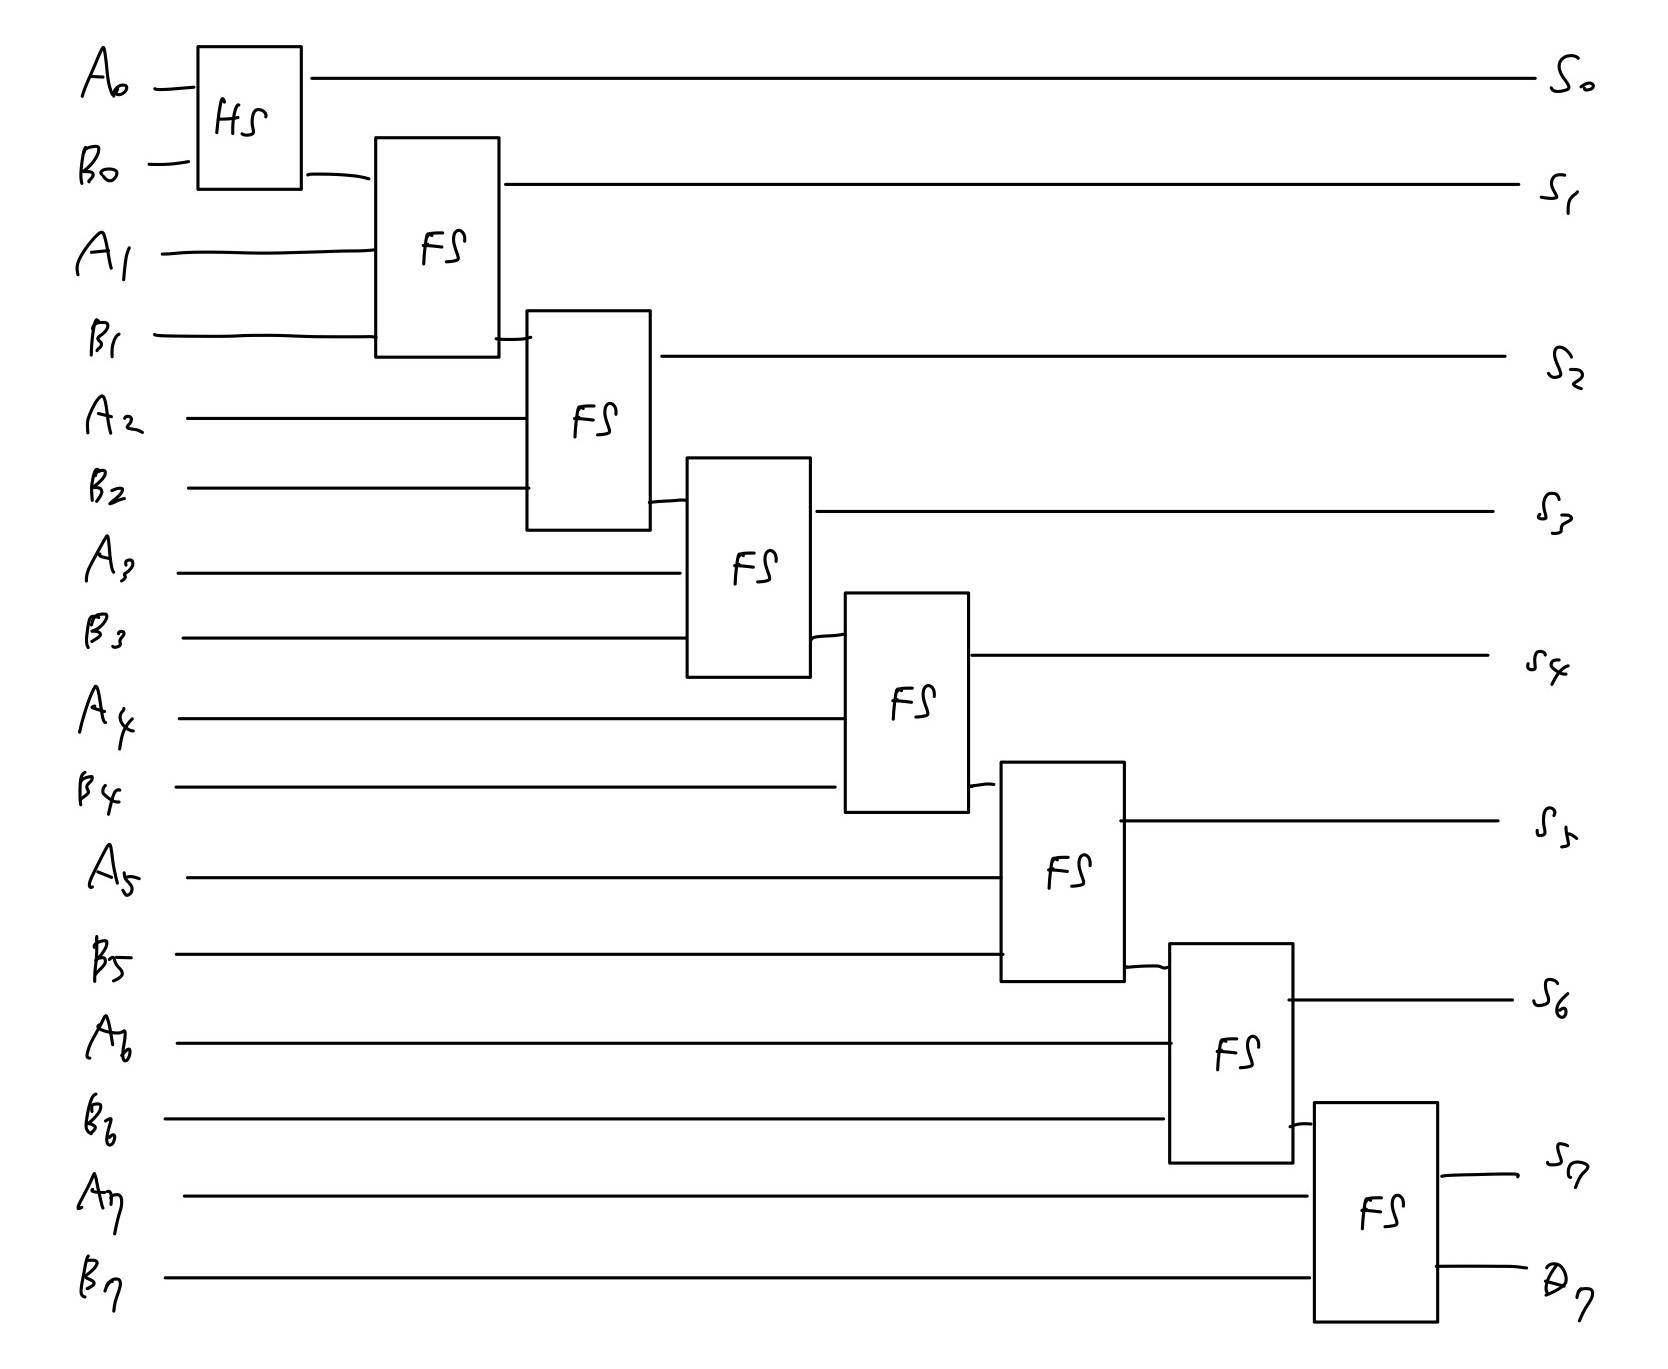
\includegraphics[width=10cm]{8bit.jpg}
  \caption{8ビット減算器の回路図.}
  \label{fig:8bit}
\end{figure}

\begin{thebibliography}{99}
  \bibitem{genzan} 【早わかり電子回路】デジタル回路の加算器・減算器をわかりやすく解説 | アイアール技術者教育研究所 | 製造業エンジニア・研究開発者のための研修/教育ソリューション.(2021).\today 閲覧.\\
  \url{https://engineer-education.com/adder-subtractor/}
\end{thebibliography}

\end{document}